% natbib guide (https://gking.harvard.edu/files/natnotes2.pdf)
% \citet     #textual citations, print the abbreviated author list
% \citet*    #textual citations, print the full author list
% \citep     #parenthetical citations, print the abbreviated author list
% \citep*    #parenthetical citations, print the full author list
% \citealt    #the same as \citet but without any parentheses.
% \citealp    #the same as \citep but without any parentheses. 
% \citeauthor{ale91}         #Alex et al.
% \citeauthor*{ale91}        #Alex, Mathew, and Ravi
% \citeyear{ale91}           #1991 
% \citeyearpar{ale91}        #(1991)

\documentclass[spanish, xcolor=dvipsnames, aspectratio=169]{beamer}

% Text encoding
\usepackage[spanish]{babel}
\usepackage[draft]{pdfcomment}
\newcommand{\pdfnote}[1]{\marginnote{\pdfcomment[icon=note]{#1}}}
% Justify text (package and function)
% \apptocmd{command}{code}{success}{failure}
\usepackage{ragged2e}
\apptocmd{\frame}{}{\justifying}{} 
% Justify text in \item
\newcommand{\itemj}{\item \justifying}

% If...else package
\usepackage{ifthen}

% Package to set transparent background image
\usepackage{tikz}

% Include image package
\usepackage{graphicx}
% Set default path for images
\graphicspath{ {./imgs/} }
% Set figure number when included
\setbeamertemplate{caption}[numbered]

% Bibliography packages
\usepackage[sort, round]{natbib}
\bibliographystyle{plainnat}

% Define colors variables
\definecolor{red}{rgb}{0.631, 0.094, 0.094} % primary color
\definecolor{grey}{rgb}{0.3686, 0.5255, 0.6235} % secondary color

% Set theme palette colors
\setbeamercolor{palette primary}{bg=red,fg=white}
\setbeamercolor{palette secondary}{bg=red,fg=white}
\setbeamercolor{palette tertiary}{bg=red,fg=white}
\setbeamercolor{palette quaternary}{bg=red,fg=white}
% strucure means itemize, enumerate, etc
\setbeamercolor{structure}{fg=red} 

% Set bibliography colors
\setbeamercolor{bibliography item}{fg=red}
\setbeamercolor{bibliography entry author}{fg=black}
\setbeamercolor{bibliography entry title}{fg=black}
\setbeamercolor{bibliography entry location}{fg=black}
\setbeamercolor{bibliography entry note}{fg=black}
% Replaces book icon in bibliography with enumeration
\setbeamertemplate{bibliography item}{[\theenumiv]}

% Table of contents style
% \setbeamertemplate{section in toc}[sections numbered]
% \setbeamertemplate{subsection in toc}[subsections numbered]
\setbeamertemplate{section in toc}[circle]
\setbeamertemplate{subsection in toc}[ball unnumbered]

% Header with navigation bar
\setbeamertemplate{headline}
{
    \leavevmode
    \hbox{
    \begin{beamercolorbox}[wd=\paperwidth,ht=2.5ex,dp=1.125ex]{palette quaternary}
    \insertsectionnavigationhorizontal{\paperwidth}{}{\hskip0pt plus1filll}
    \end{beamercolorbox} 
    }
}
% Footer with custom caption
\setbeamertemplate{footline}
{
    \leavevmode
    \hbox{
    \begin{beamercolorbox}[wd=.33\paperwidth,ht=2.6ex,dp=1ex,center]{palette quaternary}
    \usebeamerfont{author in head/foot}\insertshortauthor\hspace*{1ex}
    \end{beamercolorbox}
    \begin{beamercolorbox}[wd=.33\paperwidth,ht=2.6ex,dp=1ex,center]{palette quaternary}
    \usebeamerfont{institute in head/foot}\insertshortinstitute
    \end{beamercolorbox}
    \begin{beamercolorbox}[wd=.33\paperwidth,ht=2.6ex,dp=1ex,center]{palette quaternary}
    \insertframenumber{} / \inserttotalframenumber
    \end{beamercolorbox}}
    \vskip0pt
}

% Global Background must be put in preamble
\usebackgroundtemplate
{
    \tikz\node[opacity=0.3]{
\includegraphics[height=\paperheight, width=\paperwidth]{white_background.jpg}};
}

% One line command to print table of contents - two parameters for modes
\newcommand{\customToC}[2]
{
    \begin{frame}{Contenido}
    \tableofcontents[#1, #2]
    \end{frame}
}

% Command to plot centered figure
% Parameters: #1=image name, #2=caption 
\newcommand{\includefigure}[2]
{
    \begin{figure}[h]
    \caption{#2}
    \centering
    \includegraphics[width=0.5\textwidth]{#1}
    \end{figure}
}

% Command to set section name as variable (\renewcommand to update)
\newcommand{\sectiontitle}{}
% Command to set subsection name as variable (\renewcommand to update)
\newcommand{\subsectiontitle}{}


% Title page
\title{Minimum Makespan Scheduling and Scheduling on Identical Machines}
\subtitle{Algoritmos de aproximación, PTAS y FPTAS}
\author{Rodrigo Arévalo Gaytán \and Fausto David Hernández Jasso}
\institute{Universidad Nacional Autónoma de México}
% Date
\day=01\relax
\month=10\relax
\year=2022\relax

\begin{document}

\frame{\titlepage}

% Complete table of contents (ToC)
% \customToC{hideallsubsections}{}
\customToC{hideothersubsections}{}


%%%%%%%%%%%%%%%%% PARTE FAUSTO %%%%%%%%%%%%%%%%%%%%%%%
% Section name and highlighted ToC
\renewcommand{\sectiontitle}{Minimum Makespan Scheduling}
\section{\sectiontitle}
\customToC{currentsection,hideothersubsections}{}

\renewcommand{\subsectiontitle}{Descripción del problema}
\subsection{\subsectiontitle}

\begin{frame}{\subsectiontitle}
    \begin{itemize}
        \item Sean \(J_{1}, J_{2}, \dotsc, J_{n}\) trabajos cuyos tiempos de procesamiento son \(p_{1}, p_{2}, \dotsc, p_{n}\)
        respectivamente y un entero positivo \(m\) \textit{(el número de máquinas)}, encontrar un asignación de los 
        \(n\) trabajos a las \(m\) máquinas tal que el tiempo que se tardan en completar éstos trabajos en las máquinas
        \textbf{(que es llamado \textit{makespan})} es mínimo.
    \end{itemize}
\end{frame}

\renewcommand{\subsectiontitle}{Entendiendo el enunciado}
\subsection{\subsectiontitle}

\begin{frame}{\subsectiontitle}
    \begin{itemize}
    \item Las \(m\) máquinas son idénticas entre sí, es decir, tienen el mismo poder de cómputo.
    \item Los trabajos no pueden ser divididos entre las máquinas.
    \item Definimos al conjunto \(A_{j}\) como el conjunto de índices de los trabajos asignados a la máquina \(j\) con \(1 \leq j \leq m\).
\end{itemize}
\end{frame}

\begin{frame}{\subsectiontitle}
    \begin{itemize}
        \item Definimos a \(T_{j}\) como \(\displaystyle\sum_{i \in A_{j}} p_{i}\), notemos que \(T_{j}\) el tiempo total 
        de procesamiento que toma ejecutar todos los trabajos asignados a la máquina \(j\).
        \item Lo que debemos de encontrar es una asignación de los trabajos a las máquinas de tal manera que el \textbf{makespan}
        sea mínimo, es decir buscamos minimizar \(\mathbf{max} \ T_{j}\), para toda \(1 \leq j \leq m\).
    \end{itemize}
\end{frame}

\renewcommand{\subsectiontitle}{Algoritmo 2 aproximado}
\subsection{\subsectiontitle}

\begin{frame}{\subsectiontitle}
    Sean \(J_{1}, J_{2}, \dotsc, J_{n}\) trabajos
    \begin{itemize}
        \item Ordenamos los \(n\) trabajos de manera arbitraria. Es decir, los trabajos después de ordenarlos serán:
        \[
            J_{\sigma\left(1\right)}, J_{\sigma\left(2\right)}, \dotsc, J_{\sigma\left(n\right)}
        \]
        donde \(\sigma\) es una permutación del conjunto \(\{1, 2, \dotsc, n\}\).
        \item Ir ejecutando los \(n\) trabajos en las \(m\) máquinas en el nuevo orden de la siguiente manera:
        \begin{itemize}
            \item Sea \(J_{\sigma\left(i\right)}\) el siguiente trabajo a ejecutar con el orden obtenido en el paso anterior,
            \(J_{\sigma\left(i\right)}\) se ejecutará en el procesador que tenga la menor carga de trabajo en ese momento.
        \end{itemize}
    \end{itemize}
\end{frame}

\renewcommand{\subsectiontitle}{Cota inferior}
\subsection{\subsectiontitle}

\begin{frame}{\subsectiontitle}
    El algoritmo descrito anteriormente fue diseñado tomando en cuenta las siguientes \textbf{cotas inferiores} en la 
    solución óptima, \(\mathbf{OPT}\).
    \begin{itemize}
        \item El tiempo de procesamiento promedio de todas las máquinas el cuál es: \(\frac{1}{m}\displaystyle\sum_{i=1}^{n}p_{i}\).
        \item El tiempo de procesamiento más largo correspondiente a algún trabajo, es decir: \(\mathbf{max}\{p_{i}\}\).
    \end{itemize}
    Así sea \(\mathbf{LB}\) la cota inferior que considera ambos casos, y la definimos como sigue:
    \[
        \mathbf{LB} = \mathbf{max}\left \{ \frac{1}{m}\displaystyle\sum_{i=1}^{n}p_{i}, \mathbf{max}\{p_{i}\} \right \}
    \]
\end{frame}

\renewcommand{\subsectiontitle}{Teorema}
\subsection{\subsectiontitle}

\begin{frame}{\subsectiontitle}
    \begin{itemize}
        \item El algoritmo descrito anteriormente es un \textbf{algoritmo 2 aproximado}.
    \end{itemize}
\end{frame}

\renewcommand{\subsectiontitle}{Demostración}
\subsection{\subsectiontitle}

\begin{frame}{\subsectiontitle}
    \begin{itemize}
        \item Sea \(T\) el \textbf{makespan óptimo}, entonces notamos que \(T\) cumple con las siguientes desigualdades:
        \begin{align*}
            T &\geq \mathbf{max}\{p_{i}\} \\
            T &\geq \frac{1}{m} \sum_{j=1}^{m} T_{j} = \frac{1}{m} \sum_{i=1}^{n} p_{i}
        \end{align*}
        \item Es muy sencillo argumentar el porqué ambas desigualdades son verdaderas.
    \end{itemize}
\end{frame}

\begin{frame}{\subsectiontitle}
    Veamos \(T \geq \mathbf{max}\{p_{i}\}\)
    \begin{itemize}
        \item Por definición \(T = \mathbf{max} \ T_{j}\), para alguna \(1 \leq j \leq m\).
        \item De nuevo por definición tenemos que \(T = \mathbf{max} \displaystyle\sum_{i \in A_{j}} p_{i}\) para alguna \(1 \leq j \leq m\).
    \end{itemize}
\end{frame}

\begin{frame}{\subsectiontitle}
    Tenemos dos casos:
    \begin{itemize}
        \item \(\mathbf{max}\{p_{i}\}\) forma parte de los sumandos de \(T\), así puede ocurrir lo siguiente:
        \begin{itemize}
            \item \(T\) solamente tiene un sumando, así se tiene que se cumple \(T \geq \mathbf{max}\{p_{i}\}\), ya que en particular \(T = \mathbf{max}\{p_{i}\}\).
            \item \(T\) tiene más sumandos además de \(\mathbf{max}\{p_{i}\}\) así se tiene que se cumple \(T \geq \mathbf{max}\{p_{i}\}\), ya que en particular \(T > \mathbf{max}\{p_{i}\}\)
        \end{itemize}
        \item \(\mathbf{max}\{p_{i}\}\) no forma parte de los sumandos de \(T\), así \(p_{i}\) forma parte de alguna \(T_{k}\) tal que \(T \geq T_{k}\), así obtenemos que 
        \(T \geq \mathbf{max}\{p_{i}\}\).
    \end{itemize}
\end{frame}

\begin{frame}{\subsectiontitle}
    Veamos \(T \geq \frac{1}{m} \sum_{j}^{m} T_{j}\)
    \begin{itemize}
        \item Es inmediata ésta desigualdad.
    \end{itemize}
\end{frame}
\begin{frame}{\subsectiontitle}
    \begin{itemize}
        \item Sea \(M_{i}\) la última máquina que completa los trabajos que se le asignaron a través del algoritmo y sea \(j\) el índice del último trabajo 
        ejecutado sobre \(M_{i}\). 
        \item Entonces por construcción el máximo tiempo de procesamiento está en \(M_{i}\), es decir, \(T_{i} \geq T_{k}\) para toda \(1 \leq k \leq m\) con \(k \neq i\). 
    \end{itemize}
\end{frame}
\begin{frame}{\subsectiontitle}
    \begin{itemize}
        \item Se deduce fácilmente que la máquina \(M_{i}\) tiene la menor carga de trabajo al momento de asignar al trabajo \(J_{j}\) a ejecutarse en dicha máquina \textit{(definición del algoritmo)}. 
        \item Consecuentemente la máquina \(M_i\) tiene un tiempo de procesamiento más pequeño que el promedio.
    \end{itemize}
\end{frame}
\begin{frame}{\subsectiontitle}
    \begin{itemize}
        \item Lo que hemos dicho es que:
            \begin{align*}
                T_{i} - p_{j} &\leq \frac{1}{m}\sum_{k=1}^{n}p_{k}
            \end{align*}
        \item \(T_{i} - p_{j}\) es el momento en el cuál se asignó la ejecución del trabajo \(J_{j}\) en la máquina \(M_{i}\).
        \item Es trivial ver que:
        \begin{align*}
            p_{j} &\leq \mathbf{max}\{p_{k}\}
        \end{align*}
    \end{itemize}
\end{frame}

\begin{frame}{\subsectiontitle}
    \begin{itemize}
        \item Así
        \begin{align*}
            T_{i} &= \left(T_{i} - p_{j} \right) + p_{j} \\
                  &\leq \frac{1}{m}\sum_{k=1}^{n}p_{k} + \mathbf{max}\{p_{k}\} \\
                  &\leq T + T = 2 \cdot T
        \end{align*}
        \item Por lo tanto el algoritmo es un \textbf{algoritmo \(2\) aproximado}.
    \end{itemize}
\end{frame}

\begin{frame}{\subsectiontitle}
    \begin{figure}[H]
        \centering
        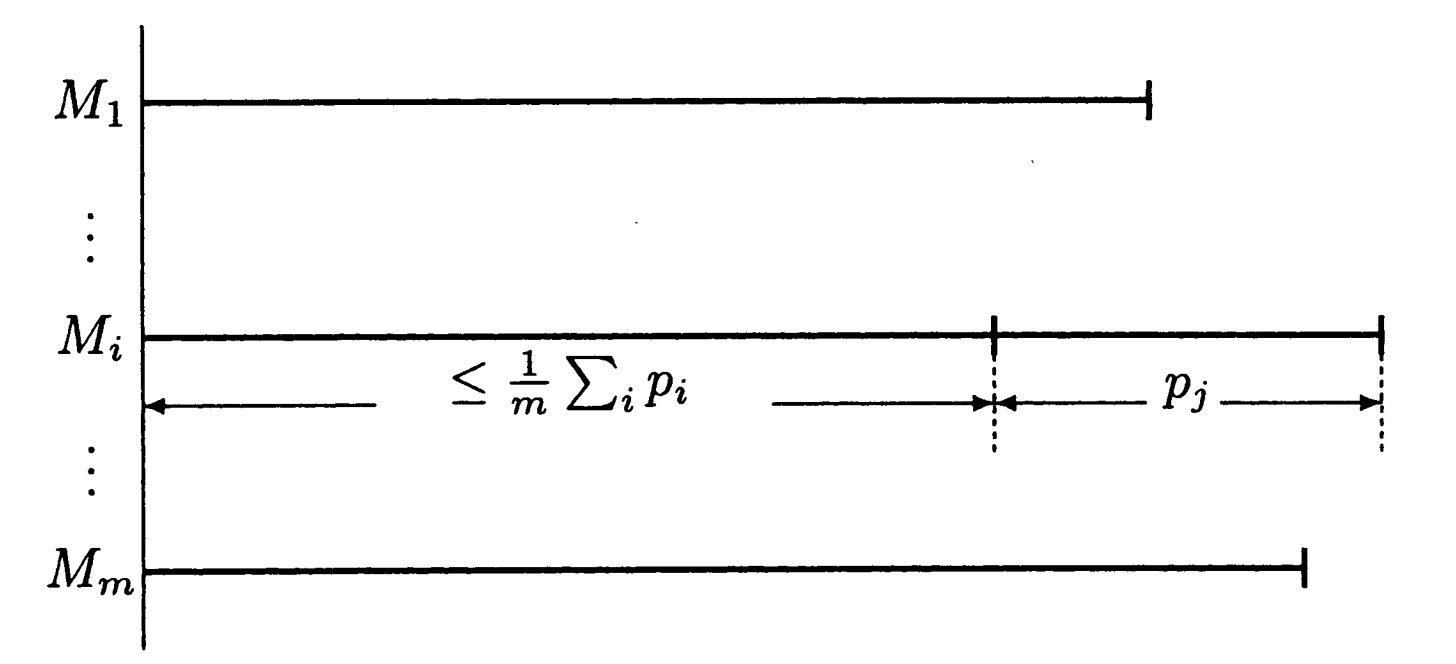
\includegraphics[scale=0.25]{imgs/MMS/img1_cc.jpg}
    \end{figure}
\end{frame}

\renewcommand{\subsectiontitle}{Ejemplo}
\subsection{\subsectiontitle}

\begin{frame}{\subsectiontitle}
    \begin{itemize}
    \item \(n = m^2 + 1\)
    \item Los trabajos son:
    \[
        J_{1}, J_{2}, \dotsc, J_{m^2 - 1}, J_{m^2}, J_{m^2 + 1}
    \]
    \item \(p_{i} = 1\) para toda \(i \in \{1, 2, \dotsc, m^2-1, m^2\}\)
    \item \(p_{m^2 + 1} = m\) 
    \item El \textbf{makespan óptimo} es \(m + 1\).
    \item El \textbf{makespan obtenido por el algoritmo} es \(2m\).
\end{itemize}
\end{frame}

\begin{frame}{\subsectiontitle}
    \textbf{Makespan óptimo}
    \begin{itemize}
        \item Notemos que el mejor de los casos sería que una máquina ejecute el trabajo \(J_{m^2 + 1}\) con un tiempo de duración de \(m\) unidades de tiempo.
        \item Así los otros \(m^2\) trabajos restantes tienen
        un tiempo de duración de una unidad de tiempo.
        \item Mientras que alguna máquina \(i\) con \(1 \leq i \leq m\) ejecuta el trabajo \(J_{m^2+1}\) las restantes \(m-1\) máquinas ejecutan cada una un trabajo con un tiempo de duración de una unidad de tiempo durante \(m\) unidades de tiempo \textit{(que es lo que dura el trabajo} \(J_{m^2+1}\) \textit{)}.
    \end{itemize}
\end{frame}

\begin{frame}{\subsectiontitle}
    \textbf{Makespan óptimo}
    \begin{itemize}
        \item Al finalizar el tiempo \(m\) los trabajos que se han ejecutados están dados por la siguiente expresión:
        \begin{align*}
            m(m-1) + 1 = m^2 - m + 1
        \end{align*}
        \item A los trabajos que nos faltan por ejecutar están dados por la expresión:
        \begin{align*}
            m^2 + 1 - ( m^2 - m + 1) &= m^2 + 1 - m^2 + m - 1 \\
            m^2 - m^2 + 1 - 1 + m &= m
        \end{align*}
        \item En éste momento contamos con \(m\) máquinas disponibles para los \(m\) trabajos así en todos los casos tenemos que \(T_{i} = m + 1\) para toda \(1 \leq i \leq m\). Por lo tanto el \textbf{makespan óptimo} es \(m + 1\).
    \end{itemize}
\end{frame}

\begin{frame}{\subsectiontitle}
    \textbf{Makespan dado por el algoritmo}
    \begin{itemize}
        \item Notemos que en el peor de los casos el algoritmo nos proporciona el siguiente orden para los trabajos:
        \[
            J_{\sigma\left(1\right)}, J_{\sigma\left(2\right)}, \dotsc, J_{\sigma\left(m^2\right)}, J_{\sigma\left(m^2+1\right)}
        \]
        con \(\sigma\) una permutación del conjunto \(\{1, 2, \dotsc, m^2, m^2 + 1\}\) y \(\sigma\left(m^2+1\right) = m^2+1\).
        \item Dado lo anterior, el último trabajo en ejecutarse es el trabajo \(J_{m^2+1}\) cuyo tiempo de duración es de \(m\) unidades de tiempo.
    \end{itemize}
\end{frame}

\begin{frame}{\subsectiontitle}
    \textbf{Makespan dado por el algoritmo}
    \begin{itemize}
        \item Por la descripción del algoritmo en las primeras \(m\) unidades de tiempo las \(m\) máquinas ejecutan en cada unidad de tiempo un trabajo cuya duración es de una unidad de tiempo así, los trabajos ejecutados hasta el tiempo \(m\) están dados por la expresión:
        \[
            m(m) = m^2  
        \]
        \item Al finalizar el tiempo \(m\), alguna de las \(m\) máquinas ejecutará el trabajo \(J_{m^2+1}\) dándonos así que el \textbf{makespan} dado por el algoritmo es de \(2m\).
    \end{itemize}
\end{frame}

\renewcommand{\subsectiontitle}{¿Es un PTAS?}
\subsection{\subsectiontitle}

\begin{frame}{\subsectiontitle}
    \begin{itemize}
        \item No es un \textbf{PTAS}\textit{(Polynomial Time Approximation Scheme)}.
    \end{itemize}
\end{frame}

%\renewcommand{\subsectiontitle}{PTAS}
%\subsection{\subsectiontitle}

%\begin{frame}{\subsectiontitle}
%    \begin{itemize}
%        \item
%    \end{itemize}
%\end{frame}

\renewcommand{\subsectiontitle}{Bin Packing}
\subsection{\subsectiontitle}

\begin{frame}{\subsectiontitle}
    \textbf{Descripción del problema}
    \begin{itemize}
        \item Dados \(n\) objetos con tamaños \(a_{1}, a_{2}, \dotsc, a_{n}\) tal que \(0 < a_{i} \leq 1\) para todo \(1 \leq i \leq n\).
        \item Encontrar un empaquetamiento en contenedores de tamaño \(1\) tal que el número de contenedores usado es el mínimo.
    \end{itemize}
\end{frame}

\begin{frame}{\subsectiontitle}
    \begin{figure}[H]
        \centering
        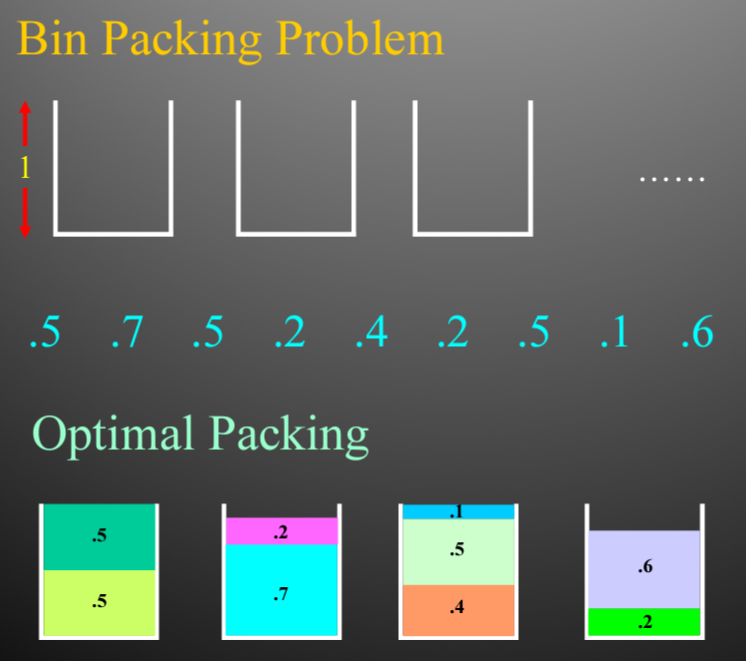
\includegraphics[scale=0.3]{imgs/MMS/img2_cc.jpg}
    \end{figure}
\end{frame}

\begin{frame}{\subsectiontitle}
    \textbf{Relación con minimum makespan scheduling}
    \begin{itemize}
        \item El problema \textbf{minimum makespan scheduling} está íntimamente relacionado con el problema de \textbf{bin packing} ya que existe una caledarización \textit{(scheduling)} con un \textbf{makespan} de tiempo \(t\) sí y solamente sí \(n\) objetos de tamaños 
        \(p_{1}, p_{2}, \dotsc, p_{n}\) pueden ser empacados en \(m\) contenedores de tamaño \(t\) cada uno. 
        \item Es decir, existe una 
        reducción del problema \textbf{minimum makespan scheduling} al problema de \textbf{bin packing}, ya que:
        \begin{itemize}
            \item De \(n\) trabajos pasamos a \(n\) objetos.
            \item De los tiempos de duración \(p_{1}, p_{2}, \dotsc, p_{n}\) correspondientes a los \(n\) trabajos pasamos a los 
            tamaños \(p_{1}, p_{2}, \dotsc, p_{n}\) de los \(n\) objetos.
            \item De \(m\) máquinas para ejecutar los trabajos pasamos a \(m\) contenedores para guardar los objetos.
            \item Del \textbf{makespan} el cual es \(t\) pasamos a que cada contenedor tenga tamaño \(t\).
        \end{itemize}
            \end{itemize}
\end{frame}

\renewcommand{\subsectiontitle}{Descripción del esquema de aproximación}
\subsection{\subsectiontitle}

\begin{frame}{\subsectiontitle}
    \textbf{Notación}
    \begin{itemize}
    \item Denotaremos al conjunto de los tamaños de los \(n\) objetos, los cuales son \(p_{1}, p_{2}, \dotsc, p_{n}\) 
    con la letra \(I\).
    \item \(\mathbf{bins}\left(I,t\right)\) es el mínimo número de contenedores de tamaño \(t\) que se necesitan 
    para empacar los \(n\) objetos.
    \item El \textbf{makespan} mínimo está dado por \(\mathbf{min}\{ \ t \ : \ \mathbf{bins}\left(I, t\right) \ \leq \ m\}\)
\end{itemize}
\end{frame}

\begin{frame}{\subsectiontitle}
    \begin{itemize}
    \item Hacemos la observación de que \(LB\) es una cota inferior y \(2 \cdot LB\) es una cota superior del \textbf{makespan} mínimo.
    \item Lo que se hará es determinar el \textbf{makespan} mínimo por búsqueda binaria en el intervalo \([LB, 2 \cdot LB]\). 
    \item El problema se puede resolver en tiempo polinomial sí el conjunto de los tamaños de los objetos es finito y su cardinalidad es fija.
\end{itemize}
\end{frame}

\begin{frame}{\subsectiontitle}
    \textbf{Bin packing con un número fijo de tamaños de los objetos.}
    \begin{itemize}
    \item Sea \(k\) el número fijo que denota los distintos tamaños de los objetos y supondremos que los contenedores tiene capacidad de \(1\).
    \item Ordenamos el tamaño de los objetos.
    \item Ahora un ejemplar genérico del problema de \textbf{bin packing} puede ser descrito de la siguiente manera:
    \begin{itemize}
        \item Una \(k-\)tupla definida como \(\left(i_{1}, i_{2}, \dotsc, i_{k}\right)\) donde cada \(i_{j}\) con \(1 \leq j \leq k\) especifica
        el número de objetos que tienen un tamaño que está en el conjunto \(I\), es decir, \(\left(i_{1}, i_{2}, \dotsc, i_{k}\right)\) especifica
        el número de de objetos de cada tamaño.
    \end{itemize}
    \item \(\mathbf{BINS}\left(i_{1}, i_{2}, \dotsc, i_{k}\right)\) denota el número mínimo de contenedores que son necesitados para empacar éstos objetos.
\end{itemize}
\end{frame}

\begin{frame}{\subsectiontitle}
    \textbf{Algoritmo de programación dinámica}
    \begin{itemize}
        \item Sea \(\left(n_{1}, n_{2}, \dotsc, n_{k}\right)\) un ejemplar del problema de \textbf{bin packing con número fijo de tamaños de los objetos} tal que 
        \(\displaystyle\sum_{i=1}^{k}n_{i} = n\)
        \item Calcularemos el conjunto \(\mathcal{Q}\) cuyos elementos serán todas las \(k-\)tuplas 
        \(\left(q_{1}, q_{2}, \dotsc, q_{k}\right)\) tales que:
        \begin{itemize}
            \item \(\mathbf{BINS}\left(q_{1}, q_{2}, \dotsc, q_{k}\right) = 1\)
            \item y además
                    \begin{align*}
                        &0 \leq q_{i} \leq n_{i} \\
                        &1 \leq i \leq k
                    \end{align*}
        \end{itemize}
    \end{itemize}
\end{frame}

\begin{frame}{\subsectiontitle}
    \begin{itemize}
        \item \(\mathcal{Q}\) contiene a lo más \(O\left(n^k\right)\) elementos, ésto es muy sencillo de ver.
        \item Denotamos como \(w_{i}\) al peso de cada uno de los \(n_{i}\) objetos.
        \item Así el peso total de los \(n_{i}\) objetos está dado por \(w_{i} \cdot n_{i}\) para toda \(1 \leq i \leq k\).
        \item Sí ocurre que:
        \[
            \left(\sum_{i = 1}^{n}  w_{i} \cdot n_{i}\right) \leq 1
        \]
        \item Entonces cualquier \(k-\)tupla \(\left(q_{1}, q_{2}, \dotsc, q_{k}\right)\) tales que:
        \begin{align*}
            &0 \leq q_{i} \leq n_{i} \\
            &1 \leq i \leq k
        \end{align*}
        cumplirá que \(\mathbf{BINS}\left(q_{1}, q_{2}, \dotsc, q_{k}\right) = 1\) 
        \item Así el número de tuplas está dado por:
        \[
            (n_{1} + 1) \cdot (n_{2} + 1) \dotsm  (n_{k-1} + 1) \cdot (n_{k} + 1)
        \]
    \end{itemize}
\end{frame}

\begin{frame}{\subsectiontitle}
    \begin{itemize}
        \item Es \(n_{i} + 1\) para toda \(1 \leq i \leq k\) ya que tenemos que contar la opción de poner el número \(0\).
        \item Tenemos que 
        \[
            n_{i} \leq n
        \]
        para toda \(1 \leq i \leq k\).
        \item Trivialmente tenemos que:
        \[
            n_{i} + 1 \leq n + 1
        \]
        para toda \(1 \leq i \leq k\).
        \item Así 
        \begin{align*}
            (n_{1} + 1) \cdot (n_{2} + 1) \dotsm (n_{k-1} + 1) \cdot (n_{k} + 1) &\leq (n + 1) \cdot (n + 1) \dotsm (n + 1) \cdot (n + 1) \\
            (n_{1} + 1) \cdot (n_{2} + 1) \dotsm (n_{k-1} + 1) \cdot (n_{k} + 1) &\leq (n + 1)^{k}
        \end{align*}
        de ahí la complejidad en tiempo.
    \end{itemize}

\end{frame}

\begin{frame}{\subsectiontitle}
    \begin{itemize}
        \item Ahora calcular todas las \(\mathbf{BINS}\left(i_{1}, i_{2}, \dotsc, i_{k}\right)\) para cada \(k-\)tupla
        \(\left(i_{1}, i_{2}, \dotsc, i_{k}\right) \in \mathcal{Q}'\) 
        \item El conjunto \(\mathcal{Q}'\) está 
        definido como sigue:
        \[
            \mathcal{Q}' = \{0, \dotsc, n_{1}\} \times \{0, \dotsm, n_{2}\}  \times \dotsm \times \{0, \dotsc, n_{k}\}  
        \]
        \item Hacemos la observación de que \(\mathbf{BINS}\left(q\right) = 1\) para todo \(q \in \mathcal{Q}\).
    \end{itemize}
\end{frame}

\begin{frame}{\subsectiontitle}
    \begin{itemize}
        \item El cálculo se hará de manera recursiva como sigue:
        \[
            \mathbf{BINS}\left(i_{1}, i_{2}, \dotsc, i_{k}\right) = 1 + \min_{q \in \mathcal{Q}} \ \mathbf{BINS}\left(i_{1} - q_{1}, i_{2} - q_{2}, \dotsc, i_{k} - q_{k}\right)
        \]
        \item Calcular cada \(\mathbf{BINS}\left(i_{1}, i_{2}, \dotsc, i_{k}\right)\) nos toma tiempo \(O\left(n^{k}\right)\) ya que de nuevo en el peor de los casos el conjunto \(\mathcal{Q}\) tiene \(O\left(n^{k}\right)\) elementos.
        \item Por lo tanto calcular todos los \(\mathbf{BINS}\left(i_{1}, i_{2}, \dotsc, i_{k}\right)\) nos toma tiempo \(O\left(n^{2k}\right)\).
        \item Al calcular todos los \(\mathbf{BINS}\left(i_{1}, i_{2}, \dotsc, i_{k}\right)\), podemos determinar \(\mathbf{BINS}\left(n_{1}, n_{2}, \dotsc, n_{k}\right)\).
    \end{itemize}
\end{frame}

\begin{frame}{\subsectiontitle}
    \begin{itemize}
        \item Podemos aceptar algunos error al calcular \textbf{minimum makespan scheduling}. Sólo hay dos formas de generar un error las cuales son:
        \begin{itemize}
            \item Redondear los tamaños de los objetos, para así tener un número acotado de los distintos tamaños de los objetos.
            \item Terminar la búsqueda binaria.
        \end{itemize}
    \end{itemize}
\end{frame}

\renewcommand{\subsectiontitle}{Core Algorithm}
\subsection{\subsectiontitle}

\begin{frame}{\subsectiontitle}
    \begin{itemize}
        \item Sea \(\varepsilon\) el parámetro de error y sea \(t\) tal que \(t \in [LB, 2 \cdot LB]\).
        \item \textbf{objeto pequeño} Un objeto es pequeño sí su tamaño es a lo más \(\varepsilon \cdot t\).
        \item Redondearemos los objetos que no son pequeños de la siguiente manera:
        \begin{itemize}
            \item Cada \(p_{j} \in [t\cdot\varepsilon\left(1 + \varepsilon\right)^{i}, t\cdot\varepsilon\left(1 + \varepsilon\right)^{i + 1}]\), 
            entonces definimos \(p_{j}'\) como \(t\varepsilon(1 + \varepsilon)^{i}\).
        \end{itemize}
        \item A lo más habrá \(k\) diferentes tamaños, donde \(k = \lceil \log_{1 + \varepsilon} \frac{1}{\varepsilon} \rceil\).
        \item Determinamos el empaquetamiento óptimo para los objetos que hemos redondeado su peso con el algoritmo de \textbf{programación dinámica} que dimos anteriormente, en contenedores de tamaño \(t\).
    \end{itemize}
\end{frame}

\begin{frame}{\subsectiontitle} 
    \begin{itemize}
        \item Como al redondear podemos reducir el tamaño de cada objeto por un factor de a lo más \(\left(1 + \varepsilon\right)\) \textit{(Ya que en el peor de los casos \(p_{j} = t\cdot\varepsilon\left(1 + \varepsilon\right)^{i + 1}\)) se convierte a \(p_{j}' = t\cdot\varepsilon\left(1 + \varepsilon\right)^{i}\)} y el factor está dado por \(\frac{p_{j}}{p_{j}'}\).
        \item Así al considerar los tamaños originales de los objetos, el empaquetamiento obtenido por el \textbf{algoritmo de programación dinámica} es válido para contenedores de tamaño \(t\left(1 + \varepsilon\right)\).
        \item Ahora empacamos los objetos pequeños de manera \textit{greedy} en los espacios que sobran en los contenedores.
        \item Denotamos \(\alpha\left(I, t, \varepsilon \right)\) como al número de contenedores usado por \textbf{Core Algorithm}.
    \end{itemize}
\end{frame}

\begin{frame}{\subsectiontitle}
    \begin{itemize}
        \item Se cumple que \(\alpha\left(I, t, \varepsilon\right) \leq \mathbf{bins}\left(I, t\right)\) ya que tenemos dos casos:
        \begin{enumerate}
            \item Sí \textbf{Core Algorithm} no utiliza nuevos contenedores para empacar los objetos pequeños entonces es trivial ver que se cumple la desigualdad.
            \item Sí \textbf{Core Algorithm} utiliza nuevos contenedores entonces todos los contenedores con excepción posiblemente del último, están llenos al menos en un tamaño \(t\) entonces al menos el empacamiento dentro de contenedores de tamaño \(t\) debió usar al menos \(\alpha\left(I, t, \varepsilon\right)\) contenedores, por lo tanto se sigue cumpliendo la desigualdad.
        \end{enumerate}
        \item Por lo anterior obtenemos que:
        \[
            \min \{ \ t \ : \ \alpha\left(I, t, \varepsilon\right) \leq m\} \leq OPT
        \]
    \end{itemize}
\end{frame}

\begin{frame}{\subsectiontitle}
    \begin{itemize}
        \item Sí \(\min \{ \ t \ : \ \alpha\left(I, t, \varepsilon\right) \leq m\}\) puede ser determinado sin error adicional durante la \textbf{búsqueda binaria}, entonces podemos usar \textbf{Core Algorithm} para obtener un \textbf{makespan} de \((1 + \varepsilon) \cdot OPT\) \textit{(debido al tamaño de los contenedores)}.
    \end{itemize}
\end{frame}

\renewcommand{\subsectiontitle}{Algoritmo $A$}
\subsection{\subsectiontitle}

\begin{frame}{\subsectiontitle}
\begin{itemize}
    \item Si \(\alpha\left(I, LB, \varepsilon\right) \leq m\), entonces usamos el empaquetamiento dado por 
    \textbf{Core Algorithm} para \(t = LB\).
    \item Si \(\alpha\left(I, LB, \varepsilon\right) > m\), entonces hacemos una \textbf{búsqueda binaria} para encontrar 
    un intervalo \([T', T]\) tal que \([T', T] \subseteq [LB, 2\cdot LB]\) con \(T - T' \leq \varepsilon \cdot LB\), 
    tal que \(\alpha\left(I, T', \varepsilon\right) > m\) y \(\alpha\left(I, T, \varepsilon\right) \leq m\). Entonces
    regresamos el empaquetamiento proporcionado por \textbf{Core Algorithm} para \(t = T\).
\end{itemize}
\end{frame}

\renewcommand{\subsectiontitle}{Teorema}
\subsection{\subsectiontitle}
\begin{frame}{\subsectiontitle}
    \begin{itemize}
        \item El algoritmo \(A\), tal que para toda \(\varepsilon > 0\), \(A\) encuentra una \textbf{caledarización} \textit{(schedule)}
        con un \textbf{makespan} de a lo más \(\left(1 + 3\cdot \varepsilon\right)\cdot OPT\). La \textbf{complejidad en tiempo} del
        algoritmo \(A\) es \(O\left(n^{2k} \cdot \lceil \log_{2} \frac{1}{\varepsilon} \rceil \right)\), donde 
        \(k = \lceil \log_{1 + \varepsilon} \frac{1}{\varepsilon} \rceil\).
    \end{itemize}   
\end{frame}

\renewcommand{\subsectiontitle}{Análisis del Algoritmo \(A\)}
\subsection{\subsectiontitle}
\begin{frame}{\subsectiontitle}
    \begin{itemize}
    \item La \textbf{búsqueda binaria} utiliza a lo más \(\lceil \log_{2} \frac{1}{\varepsilon} \rceil\) pasos, ya que 
    la \textbf{complejidad en tiempo} del algoritmo \(A\) es una hipótesis del teorema anterior.
    \item Si \(\alpha\left(I, LB, \varepsilon\right) \leq m\) entonces por las observaciones hechas tenemos que:
    \begin{align*}
        \alpha\left(I, LB, \varepsilon\right) &\leq \left(1 + \varepsilon \right) \cdot LB \\
                                                     &\leq \left(1 + \varepsilon \right) \cdot OPT \\
                                                     &\leq \left(1 + 3 \cdot \varepsilon \right) \cdot OPT
    \end{align*}
    \end{itemize}
\end{frame}

\begin{frame}{\subsectiontitle}
    \begin{itemize}
        \item Si \(\alpha\left(I, LB, \varepsilon\right) > m\) entonces tenemos que se cumple:
        \begin{itemize}
            \item \(m < \alpha\left(I, T', \varepsilon\right) \leq \mathbf{bins}\left(I, T'\right)\)
            \item \(T' \leq OPT\)
            \item y además:
            \begin{align*}
                T &\leq T' + \varepsilon \cdot LB \\
                T &\leq OPT + \varepsilon \cdot LB \\
                T &\leq OPT + \varepsilon \cdot OPT \\
                T &\leq (1 + \varepsilon) \cdot OPT
            \end{align*}
            \item Ya que \textbf{Core Algorithm} para \(T = t\) regresa una \textbf{calendarización} \textit{(schedule)}
            con un \textbf{makespan} de a lo más \((1 + \varepsilon) \cdot T\), el \textbf{makespan} de la 
            \textbf{calendarización} cumple lo siguiente:
            \begin{align*}
                (1 + \varepsilon) \cdot T &\leq  (1 + \varepsilon)^2 \cdot OPT \\
                                          &\leq  (1 + 3 \cdot \varepsilon) \cdot OPT
            \end{align*}
        \end{itemize}
    \end{itemize}
\end{frame}


%%%%%%%%%%%%%%%%%% PARTE RAG %%%%%%%%%%%%%%%%%%%%%%%%

\renewcommand{\sectiontitle}{Min Scheduling on Unrelated Parallel Machines}
\section{\sectiontitle}

\renewcommand{\subsectiontitle}{Notación de algoritmos de scheduling}
\subsection{\subsectiontitle}
\customToC{currentsection,hideothersubsections}{}

\begin{frame}{\subsectiontitle}
    Trabajos
    \begin{itemize}
        \itemj Número: $n$
        \itemj Índice: $j$
        \itemj Features:
        \begin{itemize}
            \item tiempo de procesamiento: $pj$ ó $pij$
            \item tiempo de liberación: $rj$
            \item tiempo limite: $dj$
            \item peso: $wj$
        \end{itemize}
    \end{itemize}
\end{frame}

\begin{frame}{\subsectiontitle}
    Máquinas
    \begin{itemize}
        \itemj Número: m
        \itemj Índice: i
        \itemj Ambientes:
        \begin{itemize}
            \item 1 máquina: 1
            \item Máquinas paralelas: P,P$_m$
            \item Máquinas relacionadas: Q,Q$_m$
            \item Máquinas no relacionadas: R,R$_m$        \end{itemize}
    \end{itemize}
\end{frame}

\begin{frame}{\subsectiontitle}
    Restricciones
    \begin{itemize}
        \itemj Que los trabajos tienen tiempo de liberación: rj
        \itemj Que los trabajos pueden adelantarse (preemption): pmtn
        \itemj Restricciones de precedencia: prec
        \itemj Las máquinas pueden dejar de funcionar: bkdwn
        \itemj Tamaño límite del buffer: block
         
    \end{itemize}
\end{frame}

\begin{frame}{\subsectiontitle}
    Objetivos
    \begin{itemize}
        \itemj Tiempo para completar los trabajos para cada trabajo: C$_j$
        \itemj Por retraso: L$_j$ = C$_j$ - d$_j$
        \itemj Por tardanza: T$_j$ = max L$_j$
        \itemj Y otros.
    \end{itemize}

    Ejemplos:\\
    P$||$Cmax – máquinas paralelas idénticas, minimizar la longitud de calendarización.\\
    1$|$prec, pmtn$| \Sigma w_jC_j$ - Una máquina, restricciones de precedencia y adelantamiento, minimizar la suma de los pesos de los tiempos de completud.
\end{frame}

\renewcommand{\subsectiontitle}{P $|$ pmtn $|$ C$_{max}$}
\subsection{\subsectiontitle}

\begin{frame}{\subsectiontitle}
Un límite inferior para este problema es:
\begin{align*}
    LB := max\{max_i pi,(\sum ^n_{i=1} pi)/m\}.
\end{align*}

Una calendarización que tenga este límite puede ser construida en tiempo $O(n)$ : llenar
las máquinas sucesivamente, programar los trabajos en cualquier orden y dividir
trabajos en dos partes siempre que se cumpla el límite de tiempo anterior. Programar la segunda parte de un trabajo adelantado en la siguiente máquina en el tiempo cero.

Debido al hecho de que $p_i \leq LB$ para todo $i$, las dos partes del trabajo no se traslapan.
\end{frame}

\begin{frame}
    \begin{figure}
        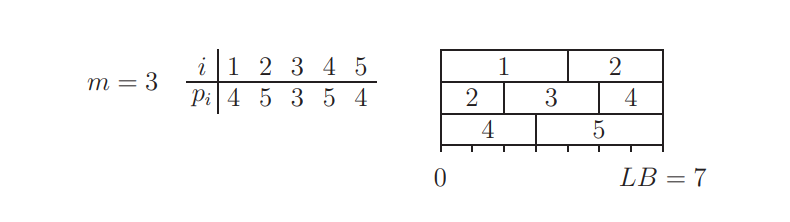
\includegraphics[width=1.1\textwidth]{imgs/mmsPTAS/pmtn-Cmax.png}
    \end{figure}
\end{frame}

\renewcommand{\subsectiontitle}{Scheduling on Unrelated Parallel Machines }
\subsection{\subsectiontitle}

\begin{frame}{\subsectiontitle}
Dado un conjunto $J$ de trabajos, un conjunto $M$ de maquinas, y por cada $j\in J$ y $i\in M$, tenemos $p_{ij}\in \mathbf{Z}^+$, que es el tiempo que se tarda en procesar el trabajo $j$ en la maquina $i$, el problema es calendarizar los trabajos en las maquinas para minimizar el makespan, es decir el tiempo de procesamiento máximo de cualquier maquina. En el libro se denota el numero de trabajos como $n$ y el numero de maquinas como $m$.\\

Nota: decimos "no relacionadas" porque no hemos supuesto ninguna relación entre los tiempos de procesamiento de un trabajo en diferentes maquinas. si cada trabajo tiene el mismo tiempo de procesamiento, sea $p_j$ dicho tiempo, en cada una de las maquinas, entonces decimos que las maquinas son \textit{identicas}.
\end{frame}

\begin{frame}{\subsectiontitle}
Para el 2-algoritmo para el problema de la programación en máquinas paralelas no relacionadas aplicaremos la técnica de poda paramétrica, junto con el redondeo de programación lineal, para obtener el algoritmo.
\end{frame}

\renewcommand{\subsectiontitle}{Poda paramétrica en una configuración de Programación Lineal}
\subsection{\subsectiontitle}

\begin{frame}{\subsectiontitle}
En este programa $x_{ij}$ es una variable indicadora que nos dice si el trabajo $j$ está programado(calendarizado) en la máquina $i$. El objetivo es minimizar $t$, el makespan. El primer conjunto de restricciones nos asegura que cada trabajo es calendarizado en una de las máquinas, y el segundo conjunto asegura que cada maquina tiene un tiempo de procesamiento de a lo más $t$.
\begin{align*}
    \texttt{minimizar } &t &\\
    \texttt{sujeto a } &\sum_{i\in M}x_{ij}=1, &j \in J\\
    &\sum_{j\in J}x_{ij}p_{ij}\leq t, &i \in M\\
    &x_{ij}\in \{0,1\}, &i \in M,j \in J\\
\end{align*}
\end{frame}

\begin{frame}{Ejemplo}
Supongamos que tenemos un solo trabajo, cuyo tiempo de procesamiento es $m$ en cada $m$ maquina. El minimo makespan es $m$. Sin embargo, la solución óptima para la relajación lineal es calendarizar el trabajo exactamente a $1/m$ en cada maquina, lo que conduce a un
valor de 1, y dando una brecha de integralidad de $m$.
\begin{figure}
        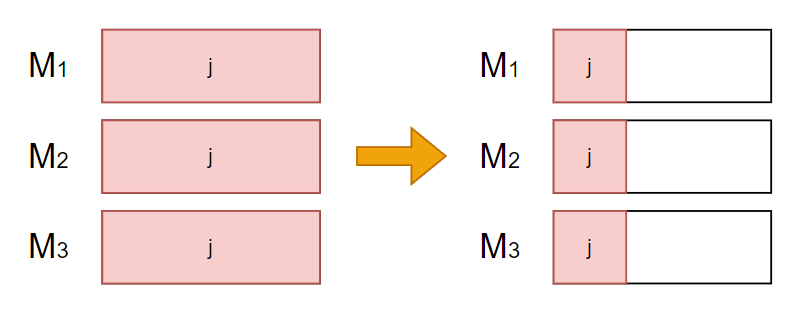
\includegraphics[width=0.8\textwidth]{imgs/mmsPTAS/ejemplojentre3.png}
    \end{figure}
\end{frame}

\begin{frame}{\subsectiontitle}
Este ejemplo ocupa una ventaja injusta que se le da por la relajación lineal. El programa entero asigna 0 a $x_{ij}$ de forma automática si $p_{ij}>t$. Pero visto de otra forma, a la relajación lineal se le tiene permitido asignar estas variables a valores que no sean 0, y de ahí obtener la solución más "barata". Esta situación podría ser rectificada si pudiéramos añadir la siguiente restricción a la relajación lineal:\\
\begin{align*}
    \forall i \in M, j\in J : \texttt{if } p_{ij}>t \texttt{ then } x_{ij} = 0.
\end{align*}
\end{frame}

\begin{frame}{\subsectiontitle}
    La restricción anterior no es una restricción lineal.\\
    Entonces para afrontar esta dificultad se usa la técnica de poda paramétrica. El parámetro será $T\in \mathbf{Z}^+$, que sera ell candidato para un limite inferior para el makespan optimo. El parámetro nos permitirá podar todos los pares máquina-trabajo tales que $p_{ij} > T$. Se define $S_T=\{(i,j)|p_{ij}\leq T\}$. Se define una familia de programas lineales $LP(T)$, una para cada valor el parámetro $T\in \mathbf{Z}^+$. $LP(T)$ usa las variables $x_{ij}$ solo para $(i,j)\in S_T$, y pregunta si hay una calendarización fraccionada y factible del makespan $\leq T$ usando las posibilidades restringidas.
    \begin{align*}
    \sum_{i:(i,j)\in S_T}x_{ij}=1, &j \in J\\
    \sum_{j:(i,j)\in S_T}x_{ij}p_{ij}\leq T, &i \in M\\
    x_{ij}\geq 0, &(i,j) \in S_T\\
\end{align*}
\end{frame}

\renewcommand{\subsectiontitle}{Propiedades de solución de punto extremo}
\subsection{\subsectiontitle}

\begin{frame}{\subsectiontitle}
Por medio de una búsqueda binaria, encontramos el valor más pequeño de $T$ tal que $LP(T)$ tiene una solución factible. Digamos que $T^*$ es este valor, $T^*$ es un limite inferior en OPT(el costo de una solución fraccionada óptima). El algoritmo redondea una solución de punto extremo a $LP(T*)$ para encontrar una calendarización con makespan $\leq 2T^*$.
\end{frame}

\begin{frame}{\subsectiontitle}
Lema 17.3: Cualquier solución de punto extremo para $LP(T)$ tiene a lo más $n+m$ variables diferentes de 0.\\

\vspace{10pt}
Demostración: Sea $r=|S_T|$ el número de variables en que $LP(T)$ está definido. Recordemos que una solución factible para $LP(T)$ es una solución de punto extremo si y sólo si corresponde a establecer $r$ restricciones linealmente independientes de $LP(T)$ para la igualdad.\\

\vspace{5pt}
De estas $r$ restricciones linealmente independientes, al menos $r-(n+m)$ deben ser elegidas a partir del tercer conjunto de restricciones (de la forma $x_{ij}\geq 0$). Las variables correspondientes se establecen con 0. Entonces, cualquier solución de punto extremo tiene a lo más $n+m$ variables distintas de 0.
\end{frame}

\begin{frame}{\subsectiontitle}
Sea $x$ una solución de punto extremo para $LP(T)$. Diremos que el trabajo $j$ es establecido de manera integral en $x$ si esta asignado de manera entera a una maquina. De otro modo diremos que $j$ está establecido de manera fraccionada.
\end{frame}

\begin{frame}{\subsectiontitle}
Corolario 17.4: Cualquier solución de punto extremo para $LP(T)$ debe establecer al menos $n-m$ trabajos de forma integral.\\

\vspace{10pt}
Demostración: Sea $x$ una solución de punto extremo para $LP(T)$, y sea $\alpha$ y $\beta$ el número de trabajos que son establecidos de manera integral y fraccionada respectivamente. Cada trabajo fraccionado está asignado al menos a 2 maquinas y así resulta en al menos 2 entradas en $x$ diferentes de 0. Así tenemos 
\begin{align*}
    \alpha + \beta = n &\alpha+2\beta \leq n+m
\end{align*}

Entonces tenemos que $\beta \leq m$ y $\alpha \geq n-m$
\end{frame}

\begin{frame}{\subsectiontitle}
    Correspondiente a una solución de punto extremo $x$ a $LP(T)$,
definimos $G = ( J, M, E)$ como la gráfica bipartita en el conjunto de vértices $J \cup M$ tal que $(j, i) \in E$ si y solo si $X_{ij} \neq 0$. Sea $F \subset J$ el conjunto de trabajos que se establecen de manera fraccionada en $x$, y sea $H$ la subgrafica de $G$ inducida en el conjunto de vértices $F\cup M$. Claramente,$( i, j )$ es una arista en $H$ si y solo si $0 < X_{ij} < 1$. Un emparejamiento en $H$ será perfecto si empareja todos los trabajos $j \in F$. El procedimiento de redondeo utiliza el hecho que la gráfica H tiene un emparejamiento perfecto.
\end{frame}

\renewcommand{\subsectiontitle}{Algoritmo de aproximación}
\subsection{\subsectiontitle}

\begin{frame}{\subsectiontitle}
\begin{enumerate}
    \item Por medio de una búsqueda binaria entre el intervalo [$\alpha/m, \alpha$], encontramos el valor más pequeño de $T\in \mathbf{Z}^+$ para el cual $LP(T)$ tiene una solución factible. Le asignamos este valor a $T^*$.%\hspace{7cm} O(nlogn)
    \item Buscamos una solución para el punto extremo, sea $x$ esta solución para $LP(T^*)$.%\hspace{6cm} O()
    \item Asignamos todos los trabajos agregados a las maquinas como con $x$.%\hspace{0.3cm} O()
    \item Construimos la gráfica $H$ y encontramos un emparejamiento perfecto $M$ en ella.%\hspace{5.1cm} O()
    \item Asignamos trabajos establecidos fraccionadamente a las máquinas acorde al emparejamiento de M.%\hspace{7.8cm} O()
\end{enumerate}
\end{frame}

\renewcommand{\subsectiontitle}{Propiedades adicionales de solución de punto extremo}
\subsection{\subsectiontitle}

\begin{frame}{\subsectiontitle}
Una gráfica conexa con su conjunto $V$ de vértices es un pseudo-arbol si contiene a lo más $|V|$ aristas. Como la gráfica es conexa tiene que tener al menos $|V|-1$ aristas. Entonces tenemos que la gráfica o es un árbol o un árbol con una arista extra. En este último caso sabemos que la gráfica tiene un solo ciclo. Digamos que una gráfica es un pseudo-bosque si cada uno de los componentes conexos de la gráfica son pseudo-arboles. 
\end{frame}

\begin{frame}{\subsectiontitle}
Lemas
\begin{enumerate}
    \item[\textbf{17.6}] La gráfica $G$ es un pseudo-bosque.
    \item[\textbf{17.7}] La gráfica $H$ tiene un emparejamiento perfecto.
    \end{enumerate}
    Teorema
    \begin{enumerate}
    \item[\textbf{17.8}] El algoritmo de aproximación nos garantiza un factor 2 para el problema de calendarizar en maquinar paralelas no relacionadas.
\end{enumerate}
\end{frame}

\begin{frame}{Lema: La gráfica $G$ es un pseudo-bosque}
Demostración:\\
En esta demostración mostramos que el número de aristas en cada componente conexo de $G$ está acotado por el número de vértices que hay en el. Entonces cada componente conexo es un pseudo-árbol.\\

\vspace{10pt}
Consideramos un componente conexo $G_C$. Restringimos $LP(T)$ y $x$ a los trabajos y maquinas de $G_C$, para obtener $LP_C(T)$ y $x_C$. Sea $x_{\overline{C}}$ el resto de $x$.\\

\vspace{5pt}
Una observación importante es que $x_C$ debe ser una solución de punto extremo para $LP_C(T)$.
\end{frame}

\begin{frame}{\subsectiontitle}
    Supongamos que este no es el caso. Entonces $x_C$ es una combinación convexa de 2 soluciones factibles para $LP_C(T)$. Cada una de estas, junto con $x_{\overline{C}}$, forman una solución factible para $LP(T)$. Así $x$ es una combinación convexa de 2 soluciones factibles para $LP(T)$. Esto nos lleva a una contradicción.\\

Aplicando el lema 17.3 (Cualquier solución de punto extremo para $LP(T)$ tiene a lo más $n+m$ variables diferentes de 0), tenemos que $G_C$ es un pseudo-árbol.
\end{frame}

\begin{frame}{Lema: H tiene emparejamiento perfecto}
Cada trabajo que se coloca en $x$ tiene exactamente una arista incidente en $G$. Eliminamos estos trabajos, junto con sus aristas incidentes, de $G$. La gráfica que nos queda es $H$. Ya que se eliminaron un mismo número de aristas y de vértices, $H$ igual es un pseudo-bosque.
\end{frame}

\begin{frame}{}
\begin{figure}
        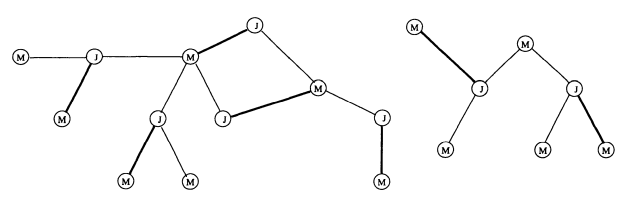
\includegraphics[width=0.9\textwidth]{imgs/mmsPTAS/graficaH.png}
    \end{figure}
\end{frame}

\begin{frame}{}
En $H$, cada trabajo tiene un grado de a lo menos 2. Entonces, todas las hojas en $H$ deben ser maquinas. Seguimos emparejando una hoja con el trabajo en el que la hoja incide, y eliminamos a ambos de la gráfica. En cada paso las hojas deben ser maquinas, al final nos quedaran ciclos pares, ya que empezamos con una gráfica bipartita. Emparejamos aristas de forma alternada en cada ciclo. Esto nos da un emparejamiento perfecto en $H$.
\end{frame}

\renewcommand{\subsectiontitle}{Garantizado factor 2 para algoritmo de aproximación}
\subsection{\subsectiontitle}

\begin{frame}{\subsectiontitle}
Demostración:\\

\vspace{10pt}
Claramente $T^*\leq$OPT, ya que $LP(OPT)$ tiene una solución factible. La solución de punto extremo, $x$, para $LP(T^*)$ tiene un makespan fraccionado $\leq T^*$. Por lo tanto, la restricción de $x$ para establecer trabajos integralmente tiene un makespan $\leq T^*$. Cada arista $(i,j)$ de $H$ satisface $p_{ij}\leq T$. El emparejamiento perfecto encontrado en $H$ calendariza a lo más un trabajo de más en cada maquina. Por lo tanto, el makespan total es $\leq 2T^* \leq 2 \cdot OPT$. El algoritmo corre en tiempo polinomial.
\end{frame}

\renewcommand{\subsectiontitle}{Ejemplo}
\subsection{\subsectiontitle}

\begin{frame}{\subsectiontitle}
Sean $m^2-m+1$ los trabajos que necesitan ser calendarizados en $m$ maquinas.
\begin{figure}
    \centering
    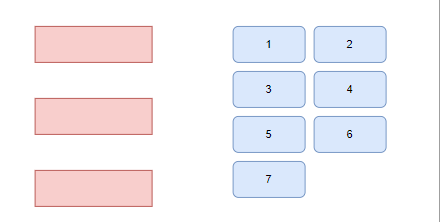
\includegraphics{imgs/mmsPTAS/EjemploMMUPM1.png}
\end{figure}
\end{frame}

\begin{frame}{\subsectiontitle}
El primer trabajo tiene un tiempo de procesamiento de $m$ en todas las maquinas, y el resto de los trabajos tienen tiempo de procesamiento unitario en cada máquina.
\begin{figure}
    \centering
    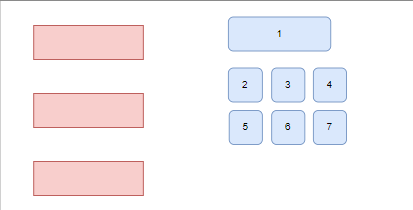
\includegraphics{imgs/mmsPTAS/EjemploMMUPM2.png}
\end{figure}
\end{frame}

\begin{frame}{\subsectiontitle}
El calendarizado optimo asigna el primer trabajo a una máquina
\begin{figure}
    \centering
    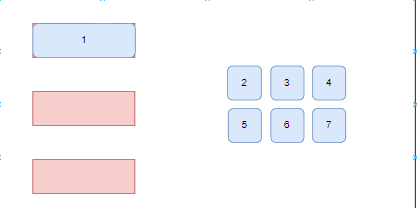
\includegraphics{imgs/mmsPTAS/EjemploMMUPM3.png}
\end{figure}
\end{frame}

\begin{frame}{\subsectiontitle}
y a los $m$ trabajos restantes a cada $m-1$ máquinas restantes.
\begin{figure}
    \centering
    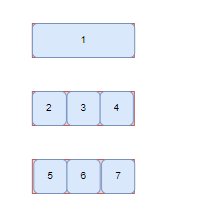
\includegraphics{imgs/mmsPTAS/EjemploMMUPM4.png}
\end{figure}
 El makespan es $m$. Es fácil ver que $LP(T)$ no tiene una solución factible para $T<m$.
\end{frame}

\begin{frame}{\subsectiontitle}
Ahora suponemos que la siguiente solución de punto extremo para $LP(T)$ es elegida. Asigna $1/m$ al primer trabajo
\begin{figure}
    \centering
    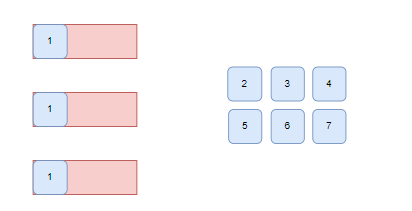
\includegraphics{imgs/mmsPTAS/EjemploMMUPM5.png}
\end{figure} y $m-1$ a los demás trabajos a cada una de las $m$ maquinas.\\

El redondeo producirá una calendarización con un makespan de $2m-1$.
\end{frame}


\begin{frame}{\subsectiontitle}
y $m-1$ a los demás trabajos a cada una de las $m$ maquinas.
\begin{figure}
    \centering
    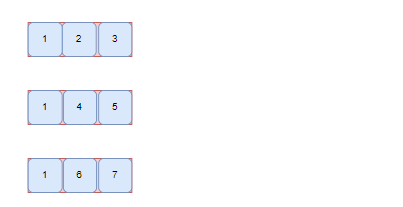
\includegraphics{imgs/mmsPTAS/EjemploMMUPM6.png}
\end{figure} 
El redondeo producirá una calendarización con un makespan de $2m-1$.
\end{frame}

%%%%%%%%%%%%%%% FIN PARTE RAG %%%%%%%%%%%%%%%%%%%%%%%
\begin{frame}[t, allowframebreaks]
\frametitle{Referencias}
\begin{thebibliography}{10}
\bibitem{vazirani2011}
\alert{Vazirani, V. V.}
\newblock  {Approximation Algorithms}
\newblock {\em Springer. Berlin (2003), 79-83, 139-144}.


\end{thebibliography}
\end{frame}

\end{document}